%
% 1_prinzip_1d.tex -- Das Prinzip der Methode der finiten Elemente in einer Dimension
%
% (c) 2024 Flurin Brechbühler, OST - Ostschweizer Fachhochschule Rapperswil
%
% !TEX root = ../../buch.tex
% !TEX encoding = UTF-8
%
\section{Prinzip in einer Dimension\label{fem:1d}}
\kopfrechts{Prinzip 1D}

Das Vorgehen zum Lösen eines Problems mit der Methode der finiten Elemente kann in fünf Schritte unterteilt werden:
\begin{enumerate}
    \item Bilden der schwachen Form
    \item Diskretisieren
    \item Aufstellen der Matrix
    \item Codieren der Anfangsbedingungen
    \item Lösen des Gleichungssystems bzw. Invertieren der Matrix
\end{enumerate}

Um die einzelnen Schritte darzustellen, betrachten wir das Problem
\begin{equation}
    u''(x) = f(x)
    \label{fem:1d:poisson_gleichung},
\end{equation}
was der Poisson-Gleichung entspricht. 
Diese findet in vielen Teilen der Physik Anwendung und ist gleichzeitig ein gutes, einfaches Beispiel einer mit der FEM lösbaren Differenzialgleichung.
Si soll im ganzen Definitionsbereich
\begin{equation}
    l = [a,b]
\end{equation}
gelten.


\subsection{Bilden der schwachen Form}
Um das Problem in die schwache Form zu bringen, wird über beide Seiten der Poisson-Gleichung \ref{fem:1d:poisson_gleichung} integriert.
Zuvor werden jedoch beide Seiten mit der Testfunktion $ v(x) $ multipliziert.
Diese wird definiert als eine beliebige Funktion $ v \colon \mathbb{R} \rightarrow \mathbb{R} $.
Die resultierende Gleichung
\begin{equation}
    \int_l(u''(x) \cdot v(x)) \diff x = \int_l(f(x) \cdot v(x)) \diff x \myforall v(x)
    \label{fem:1d:schwache_form}
\end{equation}
sollte einem bekannt vorkommen, denn sie entsteht auch beim Herleiten der ersten Variation.
Im Kapitel \ref{buch:variation:section:fundamentallemma} zum Fundamentallemma wird bewiesen, dass die beiden Ausdrücke \eqref{fem:1d:poisson_gleichung} und \eqref{fem:1d:schwache_form} gleichwertig sind.

Durch partielles Integrieren der linken Seite kann die Ordnung der Differenzialgleichung um eins verringert werden:
\begin{align}
    \int_l f(x) \cdot v(x) \diff x &= \int_l u''(x) \cdot v(x) \diff x \\
                                 &= \left[ u'(x) \cdot v(x) \right]_{a}^{b} - \int_l u'(x) \cdot v'(x) \diff x \\
                                 &= - \int_l u'(x) \cdot v'(x) \diff x \\
                                 &= - \Phi(u, v),
\end{align}
wobei der Term
\begin{equation}
    \left[ u'(x) \cdot v(x) \right]_{a}^{b}
\end{equation}
Null ist, wenn die Funktion $u'(x)$ die Randbedingung
\begin{equation}
    u'(a) = u'(b) = 0
\end{equation}
erfüllt. 

Der erhaltene Term wird als $-\Phi(u, v)$ abgekürzt.
Dieser Weg kann abhängig von der ursprünglichen Differenzialgleichung variieren.
Das häufigste Vorgehen, das partielle Ableiten der rechten Seite, wurde hier jedoch gezeigt.
Ziel ist es, die Ordnung der Differenzialgleichung möglichst stark zu verkleinern, da so Ansätze kleinerer Ordnung verwendet werden können.
Dies spart Rechenleistung.


\subsection{Diskretisieren\label{fem:1d:diskretisieren}}
Ziel des Diskretisierens ist es, das unendlichdimensionale Problem in ein endlichdimensionales umzuwandeln.
Dazu werden die ursprünglichen Funktionen $u(x)$, $f(x)$ und $v(x)$ an $N$ verschiedenen Punkten $x_n$ abgetastet.
Die resultierenden Knotenvariablen
\begin{equation}
    u_n = u(x_n) 
    \text{,} \quad
    f_n = f(x_n)
    \quad \text{und} \quad
    v_n = v(x_n)
\end{equation}
können dann mit einer stetigen Interpolationsfunktion mit schmalem Träger
\begin{equation}
    a_n(x) = \left\{ \begin{array}{ll}
        1
            & \text{für} \quad x = x_n \\
        a(x) \in (0, 1) 
            & \text{für} \quad x_{n-1} < x < x_n \quad \text{und} \quad x_n < x < x_{n+1} \\
        0
            & \text{sonst} 
    \end{array} \right.
\end{equation}
multipliziert werden und zu einer durch $N$ Werte parametrisierten stetigen Funktion zusammengesetzt werden:
\begin{equation}
    u(x) \approx \sum_{n=0}^{N}{u_n \cdot a_n(x)} 
    \text{,} \quad
    f(x) \approx \sum_{n=0}^{N}{f_n \cdot a_n(x)} 
    \quad \text{und} \quad
    v(x) \approx \sum_{n=0}^{N}{v_n \cdot a_n(x)}.
\end{equation}
Dies funktioniert, da die Formfunktionen so gewählt wurden, dass an den Stützstellen jeweils nur eine der Formfunktionen von Null verschieden ist.
Dabei hat die Formfunktion an ebendieser Stützstelle den Wert Eins.
Das führt dazu, dass die interpolierte Funktion, die aus der Summe der einzelnen skalierten Formfunktionen entsteht, in den Stützstellen die gleichen Werte aufweist wie die ursprüngliche Funktion.

Die Formfunktionen sollten zudem eine Zerlegung von Eins bilden
\begin{equation}
    \sum_{n} a_n(x) = 1, \label{fem:1d:zerlegung_v_eins}
\end{equation}
sodass konstante Triviallösungen exakt repräsentiert werden können.

Für die Interpolationsfunktion $a(x)$ können verschiedene Ansätze gewählt werden:
\begin{itemize}
    \item[\textbf{linear:}] 
        Einfach zu rechnen und zu verstehen, jedoch ist die erste Ableitung unstetig und die zweite Ableitung Null.
        Dementsprechend kann dieser Ansatz nur verwendet werden, wenn keine zweiten Ableitungen im vereinfachten Problem vorkommen.
    \item[\textbf{quadratisch:}]
        Ist die Ordnung des Problems um eins zu hoch, um den linearen Ansatz zu verwenden, kann der quadratische Ansatz eingesetzt werden.
        Dieser besitzt nämlich eine zweite Ableitung ungleich Null.
        Die erste Ableitung ist jedoch nach wie vor unstetig, was zu nicht sehr schönen Resultaten führt.
    \item[\textbf{kubisch:}]  
        Der kubische Ansatz hat sehr gute Eigenschaften: 
        Er besitzt eine stetige erste Ableitung sowie zweite und dritte Ableitungen ungleich Null. 
        Zudem bietet er die Möglichkeit, die ersten Ableitungen der Zielfunktion an den Stützpunkten frei zu wählen.
        Dies wird später zum Berücksichtigen der Anfangsbedingungen hilfreich sein.
\end{itemize}

\subsubsection{Linearer Ansatz}
%
% linearer_ansatz.tex
%
% (c) 2024 Flurin Brechbühler
%
\begin{figure}
    \centering
    \subfloat[Formfunktion des linearen Ansatzes]{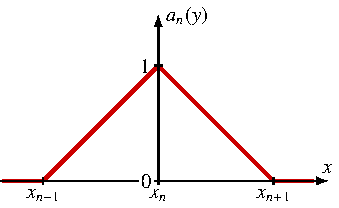
\includegraphics{papers/fem/images/linear_formfkt.pdf}\label{fem:1d:abb:linear:formfkt}}
    \hfill
    \subfloat[Skalierte Formfunktionen mit der zu interpolierenden Funktion $f(x)$]{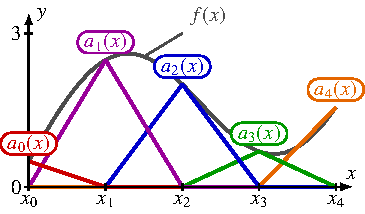
\includegraphics{papers/fem/images/linear_formfkt_skaliert.pdf}\label{fem:1d:abb:linear:skaliert}}

    \subfloat[Gegenüberstellung der interpolierten und der uhrsprünglichen Funktion.]{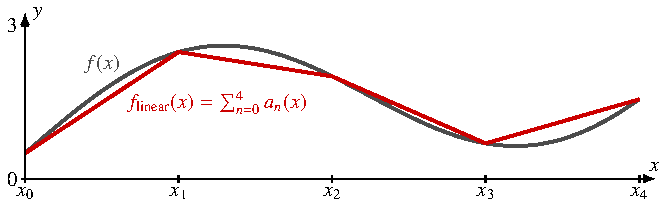
\includegraphics{papers/fem/images/linear_interpoliert.pdf}\label{fem:1d:abb:linear:vergleich}}
    \caption{Lineare Interpolation des Signals $f(x)$.}
    \label{fem:1d:abb:linear}
\end{figure}
    
Der lineare Ansatz verwendet die in Abbildung \ref{fem:1d:abb:linear:formfkt} gezeigten linearen Funktionen
\begin{equation}
    \def\arraystretch{\formfktStretch}
    a_n(x) = \left\{ \begin{array}{ccc}
        1+\frac{x-x_n}{x_n - x_{n-1}} 
            & \text{für} & x_{n-1} < x < x_n \\

        1-\frac{x-x_n}{x_{n+1} - x_n} 
            & \text{für} & x_n \leq x < x_{n+1} \\

        0
            & \text{sonst}
    \end{array} \right..
\end{equation}
Diese Formfunktionen können mit dem Ansatz 
\begin{equation}
    a_n(x) = c_1x + c_0
\end{equation}
und den zu erfüllenden Bedingungen
\begin{equation}
        a_n(x_n) = 1 
        \quad \text{und} \quad
        a_n(x_{n-1}) = a(x_{n+1}) = 0
\end{equation}
hergeleitet werden.

Die interpolierte Funktion $f_\text{linear} (x)$ folgt der vorgegebenen Funktion $f(x)$ nicht sehr präzise.
Es ist also naheliegend, dass für eine bestimmte Menge Stützstellen mit dem linearen Ansatz nur bedingt genaue Resultate folgen werden.

\subsubsection{Quadratischer Ansatz}
%
% quadratischer_ansatz.tex
%
% (c) 2024 Flurin Brechbühler
%
\begin{figure}
    \centering
    \subfloat[Formfunktionen des quadratischen Ansatzes]{
        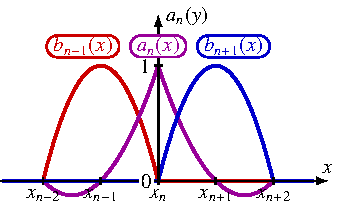
\includegraphics[scale=0.95,valign=t]{papers/fem/images/quadratisch_formfkt.pdf}
        \vphantom{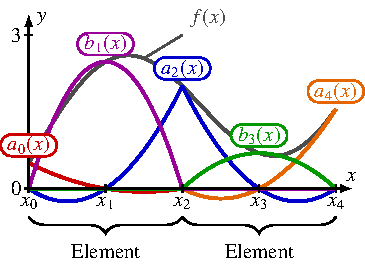
\includegraphics[width=0.45\textwidth,valign=t]{papers/fem/images/quadratisch_formfkt_skaliert.pdf}}
        \label{fem:1d:abb:quadratisch:formfkt}
    }
    \hfill
    \subfloat[Skalierte Formfunktionen mit der zu interpolierenden Funktion $f(x)$]{
        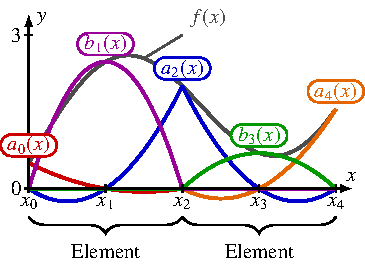
\includegraphics[scale=0.95,valign=t]{papers/fem/images/quadratisch_formfkt_skaliert.pdf}
        \vphantom{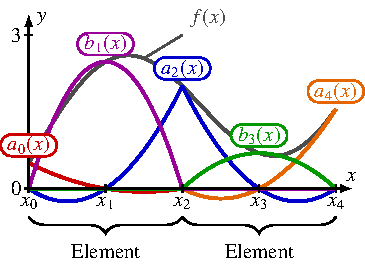
\includegraphics[width=0.45\textwidth,valign=t]{papers/fem/images/quadratisch_formfkt_skaliert.pdf}}
        \label{fem:1d:abb:quadratisch:skaliert}
    }

    \subfloat[Gegenüberstellung der interpolierten und der ursprünglichen Funktion.]{
        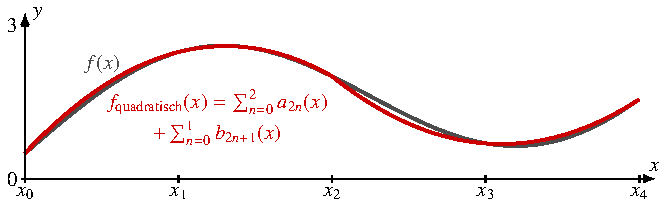
\includegraphics[scale=0.95]{papers/fem/images/quadratisch_interpoliert.pdf}
        \label{fem:1d:abb:quadratisch:vergleich}
    }
    \caption{Quadratische Interpolation des Signals $f(x)$.}
    \label{fem:1d:abb:quadratisch}
\end{figure}
     
Für das Interpolieren mit dem quadratischen Ansatz muss das Vorgehen leicht angepasst werden, da sonst die Bedingung \ref{fem:1d:zerlegung_v_eins} nicht erfüllt wird. 
Wie beim eindimensionalen Fall werden im Definitionsbereich Knotenpunkte definiert und diese mit Elementen verbunden.
Pro Element wird nun ein weiterer Knoten definiert. 
Dieser wird oft in der Mitte des Elements gewählt und erhält seine eigene Formfunktion.
Die Elemente werden anschliessend wieder durchnummeriert.

Die in Abbildung \ref{fem:1d:abb:quadratisch:formfkt} gezeigten Formfunktionen lauten
\begin{equation}
    \def\arraystretch{\formfktStretch}
    a_n(x) = \left\{ \begin{array}{ccc}
         \frac{1}{2} \left(\frac{x-x_{n-1}}{x_{n-2}-x_{n-1}}\right)^2 
        -\frac{1}{2}       \frac{x-x_{n-1}}{x_{n-2}-x_{n-1}}
            & \text{für} & x_{n-2} \leq x < x_{n-1} \\
        
         \frac{1}{2} \left(\frac{x-x_{n  }}{x_{n-1}-x_{n  }}\right)^2 
        -\frac{3}{2}       \frac{x-x_{n  }}{x_{n-1}-x_{n  }} 
        +1  
            & \text{für} & x_{n-1} \leq x < x_n \\
        
         \frac{1}{2} \left(\frac{x-x_{n  }}{x_{n+1}-x_{n  }}\right)^2 
        -\frac{3}{2}       \frac{x-x_{n  }}{x_{n+1}-x_{n  }} 
        +1  
            & \text{für} & x_{n-1} \leq x < x_n \\
        
         \frac{1}{2} \left(\frac{x-x_{n+1}}{x_{n+2}-x_{n+1}}\right)^2 
        -\frac{1}{2}       \frac{x-x_{n+1}}{x_{n+2}-x_{n+1}}
            & \text{für} & x_{n-1} \leq x < x_n \\
        
        0
            & \text{sonst}
    \end{array} \right.
\end{equation}
für die Knoten an den Enden der Elemente und
\begin{equation}
    \def\arraystretch{\formfktStretch}
    b_n(x) = \left\{ \begin{array}{ccc}
        -\left(\frac{x-x_{n}}{x_{n}-x_{n-1}}\right)^2+1
            & \text{für} & x_{n-1} < x < x_n \\

        -\left(\frac{x-x_{n}}{x_{n}-x_{n+1}}\right)^2+1
            & \text{für} & x_n \leq x < x_{n+1} \\

        0 
            & \text{sonst}
    \end{array} \right.
\end{equation}
für die Knoten in der Mitte der Elemente.

Diese Formfunktionen können mit den Ansätzen 
\begin{equation}
    a_n(x) = c_2x^2 + c_1x + c_0
    \quad \text{bzw.} \quad
    b_n(x) = d_2x^2 + d_1x + d_0
\end{equation}
und den Bedingungen 
\begin{equation}
    a_n(x_n) = 1 
    \quad \text{und} \quad 
    a_n(x_{n-2}) = a_n(x_{n-1}) = a_n(x_{n+1}) = a_n(x_{n+2}) = 0
\end{equation}
für Knotenpunkte am Ende der Elemente bzw.
\begin{equation}
    b_n(x_n) = 1
    \quad \text{und} \quad 
    b_n(x_{n-1}) = b_n(x_{n+1}) = 0
\end{equation}
für Knotenpunkte in der Mitte der Elemente hergeleitet werden.
Dabei ist zu beachten, dass die Formfunktionen $a_n(x)$ aus zwei quadratischen Funktionen zusammensetzen: 
Eine für den Bereich $x_{n-2} \leq x \leq x_n$ und eine für den Bereich $x_n \leq x \leq x_{n+2}$.

Die resultierende interpolierte Funktion $f_\text{quadratisch} (x)$, gezeigt in Abbildung \ref{fem:1d:abb:quadratisch:vergleich}, folgt der vorgegebenen Funktion $f(x)$ schon viel besser als im linearen Fall.
Es äussert sich jedoch auch eine Schwäche des quadratischen Ansatzes: 
An der Stützstelle $x_2$ ist aufgrund der unstetigen Ableitung von $f_\text{quadratisch}$ ein leichter Knick zu erkennen.
Dies ist nicht besonders schön.
Abhilfe schafft der kubische Ansatz.

\subsubsection{Kubischer Ansatz}
%
% linearer_ansatz.tex -- Formfunktionen linearer Ansatz
%
% (c) 2024 Flurin Brechbühler
%
\documentclass[tikz]{standalone}
\usepackage{amsmath}
\usepackage{times}
\usepackage{txfonts}
\usepackage{pgfplots}
\usepackage{csvsimple}

\usetikzlibrary{arrows,intersections,math}
\definecolor{darkred}{rgb}{0.8,0,0}
\definecolor{darkpurple}{rgb}{0.6,0,0.6}
\definecolor{darkblue}{rgb}{0,0,0.8}
\definecolor{darkgreen}{rgb}{0,0.6,0}

\begin{document}
\def\skala{1}

\begin{tikzpicture}[>=latex,thick,scale=\skala]
\begin{scope}

% Plots
	% a_n
\draw[color=darkred,line width=1.4pt] plot[domain=-1.025:-1, scale=4, smooth]
({\x},{0});
\draw[color=darkred,line width=1.4pt] plot[domain=-1:0, scale=4, smooth]
({\x},{(1-2*\x)*(\x+1)^2});
\draw[color=darkred,line width=1.4pt] plot[domain=0:1, scale=4, smooth]
({\x},{(1+2*\x)*(1-\x)^2});
\draw[color=darkred,line width=1.4pt] plot[domain=1:1.025, scale=4, smooth]
({\x},{0});
	% b_n
\draw[color=darkpurple,line width=1.4pt] plot[domain=-1.025:-1, scale=4, smooth]
({\x},{0});
\draw[color=darkpurple,line width=1.4pt] plot[domain=-1:0, scale=4, smooth]
({\x},{\x*(\x+1)^2});
\draw[color=darkpurple,line width=1.4pt] plot[domain=0:1, scale=4, smooth]
({\x},{\x*(1-\x)^2});
\draw[color=darkpurple,line width=1.4pt] plot[domain=1:1.025, scale=4, smooth]
({\x},{0});

% x-Achse
\draw[->] (-4.1,0) -- (4.4,0) coordinate[label={$x$}];
\draw (4,-0.1) -- (4,0.1);
\draw (-4,-0.1) -- (-4,0.1);
\node at (-4,0) [below] {$x_{n-1}$};
\node at ( 0,0) [below] {$x_n$};
\node at ( 4,0) [below] {$x_{n+1}$};

% y-Achse
\draw[->] (0,{-0.1}) -- (0,{4.3})
coordinate[label={right:$y$}];
\node at (-0.1,0) [left, inner sep=1pt, fill=white, rounded corners] {$0$};
\draw (-0.1,4) -- (0.1,4);
\node at (0,4) [left] {$1$};

\end{scope}
\end{tikzpicture}
\end{document}

Der kubische Ansatz bringt die Möglichkeit, den Wert der Funktion wie auch den Wert der Ableitung an den Stützstellen frei zu wählen.
Dafür muss der Ansatz etwas erweitert werden:
\begin{equation}
    u(x) \approx \sum_{n}{u_n \cdot a_n(x)} \rightarrow u(x) \approx \sum_{n}{u_n \cdot a_n(x) + u'_n \cdot b_n(x)}.
\end{equation}

Die Formfunktionen 
\begin{equation}
    \def\arraystretch{\formfktStretch}
    a(x) = \left\{ \begin{array}{ccc}
        - 2 \cdot \left(\frac{x-x_{n-1}}{x_n-x_{n-1}}\right)^3 
        + 3 \cdot \left(\frac{x-x_{n-1}}{x_n-x_{n-1}}\right)^2 
            & \text{für} & x_{n-1} < x < x_n \\

        - 2 \cdot \left(\frac{x-x_{n+1}}{x_n-x_{n+1}}\right)^3 
        + 3 \cdot \left(\frac{x-x_{n+1}}{x_n-x_{n+1}}\right)^2 
            & \text{für} & x_n \leq x < x_{n+1} \\

        0
            & \text{sonst}
    \end{array} \right.
\end{equation}
und
\begin{equation}
    b(x) = \left\{ \begin{array}{ccc}
          \left(\frac{(x-x_{n-1})^3}{(x_n-x_{n-1})^2}\right)
        - \left(\frac{(x-x_{n-1})^2}{x_n-x_{n-1}}\right)
            & \text{für} \quad x_{n-1} < x < x_n \\

          \left(\frac{(x-x_{n+1})^3}{(x_n-x_{n+1})^2}\right)
        - \left(\frac{(x-x_{n+1})^2}{x_n-x_{n+1}}\right)
            & \text{für} \quad x_n \leq x < x_{n+1} \\

        0
            & \text{sonst}
    \end{array} \right.
\end{equation}
dargestellt in Abbildung \ref{fem:1d:abb:kubisch:formfkt}, können mit dem Ansatz
\begin{equation}
    a(x) = c_3x^3 + c_2x^2 + c_1x + c_0 
    \quad \text{bzw.} \quad
    b(x) = d_3x^3 + d_2x^2 + d_1x + d_0
\end{equation}
und den Bedingungen 
\begin{equation}
        a(x_n) = 1 
        \quad \text{und} \quad
        a(x_{n-1}) = a(x_{n+1}) = 0 
        \quad \text{sowie} \quad
        a'(x_{n-1}) = a'(x_n) = a'(x_{n+1}) = 0
\end{equation}
und
\begin{equation}
        b'(x_n) = 1 
        \quad \text{und} \quad
        b'(x_{n-1}) = b'(x_{n+1}) = 0 
        \quad \text{sowie} \quad
        b(x_{n-1}) = b(x_n) = b(x_{n+1}) = 0
\end{equation}
hergeleitet werden.

Die durch diese Funktionen interpolierte Funktion $f_\text{kubisch} (x)$ ist wie in Abbildung \ref{fem:1d:abb:kubisch:vergleich} zu sehen ist kaum mehr von der ursprünglichen Funktion $f(x)$ zu unterscheiden.
Dass der kubische Ansatz gute Resultate liefert, war zu erwarten, denn die Formfunktionen entsprechen den in Kapitel \ref{buch:nichtdiff:section:splines} hergeleiteten Hermite-Polynomen.


\subsection{Erstellen der Matrix\label{fem:1d:matrix_erstellen}}
Um das Problem als Matrixgleichung zu repräsentieren, muss zunächst die Differenzialgleichung in der schwachen Form in ein lineares Gleichungssystem überführt werden.
Mit den Approximationen 
\begin{align}
    u(x) &\approx \sum_i u_i \cdot a_i(x) \\
    f(x) &\approx \sum_i f_i \cdot a_i(x) \\
    v(x) &\approx \sum_j v_j \cdot a_j(x)
\end{align}
aus der Diskretisierung kann die schwache Form der Differenzialgleichung 
\begin{equation}
    - \int_l u'(x) \cdot v'(x) \diff x = \int_l f(x) \cdot v(x) \diff x
\end{equation}
als
\begin{equation}
    - \int_l \biggl(\sum_i u_i \cdot a'_i(x)\biggr) \biggl(\sum_j v_j \cdot a'_j(x)\biggr) \diff x 
    = \int_l \biggl(\sum_i f_i \cdot a_i(x) \biggr) \biggl(\sum_j v_j \cdot a_j(x) \biggr) \diff x 
    \myforall v_i
\end{equation}
geschrieben werden.
Die vorherige Gleichung kann zu
\begin{equation}
    - \int_l \sum_i u_i \cdot a'_i(x) \cdot a'_j(x) \diff x = \int_l \sum_i f_i \cdot a_i(x) \cdot a_j(x) \diff x \myforall j
\end{equation}
vereinfacht werden.
Dabei wird die Menge der Testfunktionen reduziert.
Um nicht alle Testfunktionen mit beliebig breitem Träger berücksichtigen zu müssen, werden nur die $N$ verschiedenen Testfunktionen mit schmalstmöglichem Träger verwendet.
Da alle anderen Testfunktionen aus diesen ``zusammengebaut'' werden können, ist die Gleichung auch für diese erfüllt.
Diese Vereinfachung ermöglicht es, die Summen aus den Integralen zu bringen und die Gleichung als
\begin{equation}
    - \sum_i u_i \underbrace{\int_l a'_i(x) \cdot a'_j(x) \diff x}_{l_{ij}} = \sum_i f_i \underbrace{\int_l a_i(x) \cdot a_j(x) \diff x}_{l_{ij}} \myforall j \label{papers:fem:prinzip1d:finale_gleichung}
\end{equation}
zu schreiben.
Übrig bleibt also, da die Integrale ausgewertet werden können, ein lineares Gleichungssystem mit $N$ Unbekannten $u_i$ und $N$ Gleichungen (eine pro $j$). 

Das erhaltene Gleichungssystem lässt sich nun sehr gut als Matrizen, bei denen die Zeilen über $i$ und die Spalten über $j$ iterieren, darstellen:
\begin{multline}
    -\left(
        \begin{matrix}
            \int_l a'_1(x) \cdot a'_1(x) \diff x & \hdots & \int_l a'_N(x) \cdot a'_1(x) \diff x \\
            \vdots                               & \ddots & \vdots                               \\
            \int_l a'_1(x) \cdot a'_N(x) \diff x & \hdots & \int_l a'_N(x) \cdot a'_N(x) \diff x \\
        \end{matrix}
    \right)
    \left(
        \begin{matrix}
            u_1 \\
            \vdots \\
            u_N
        \end{matrix}
    \right) \\
    = \\
    \left(
        \begin{matrix}
            \int_l a_1(x) \cdot a_1(x) \diff x & \hdots & \int_l a_N(x) \cdot a_1(x) \diff x \\
            \vdots                             & \ddots & \vdots                             \\
            \int_l a_1(x) \cdot a_N(x) \diff x & \hdots & \int_l a_N(x) \cdot a_N(x) \diff x \\
        \end{matrix}
    \right)
    \left(
        \begin{matrix}
            f_1 \\
            \vdots \\
            f_N
        \end{matrix}
    \right),
\end{multline}
was kompakt als
\begin{equation}
    -\mathbf{L}\vec{u} = \mathbf{M}\vec{f}
\end{equation}
geschrieben wird.
Auch gängig ist das Zusammenfassen von $\mathbf{M}\vec{f}$ zu $\vec{b}$, was zur Gleichung
\begin{equation}
    \mathbf{L}\vec{u} + \vec{b} = 0
\end{equation}
führt.

$\mathbf{L}$ wird aufgrund des schmalen Trägers der Funktionen $a_n(x)$ (sowie $b_n(x)$ beim kubischen Ansatz) sehr schwach besetzt sein, da viele der Integrale
\begin{equation}
    \quad \int_l a'_i(x) \cdot a'_j(x) \diff x 
\end{equation}
Null sein werden.
Von Null verschieden sind nur die Einträge, deren zugehörige Datenpunkte nebeneinander liegen.
Die Matrix ist also symmetrisch, da es keine Rolle spielt in welcher Reihenfolge man die Testfunktionen multipliziert.
Da $\mathbf{L}$ die Gram-Matrix\footnote{Mehr über die Gram-Matrix im Buch Lineare Algebra: Eine anwendungsorientierte Einführung \cite{buch:linalg}.} des Skalarprodukts darstellt und das Skalarprodukt positiv definit ist, ist auch $\mathbf{L}$ positiv definit.

\subsubsection{Kubischer Ansatz}
Auch hier verlangt der kubische Ansatz mit seinen zwei Funktionen pro Datenpunkt eine leichte Anpassung: 
\begin{itemize}
    \item Die Vektoren $\vec{b}$ und $\vec{f}$ werden für die gleiche Menge Datenpunkte doppelt so viele Elemente enthalten.
          Dies aus dem Grund, dass für jeden Wert $u_i$ ein zweiter Wert $u'_i$ dazukommt.
    \item Folglich wird die Matrix $\mathbf{L}$ doppelt so viele Zeilen und Spalten enthalten. 
\end{itemize}


\subsection{Codieren der Anfangsbedingungen\label{fem:1d:anfangsbedingungen}}
Wir betrachten das Gleichungssystem in der Form 
\begin{equation}
    \mathbf{L}\vec{u} = -\vec{b}. 
    \label{fem:1d:gleichungssystem}
\end{equation}
Dieses kann, um die kommenden Schritte besser verständlich zu machen, in einem Gauss-Tableau als
\begin{equation}
    \begin{array}{|ccccc|c|}
        \hline
        l_{11} & l_{12} & l_{13} & \cdots & l_{1N} & -b_1   \\
        l_{21} & l_{22} & l_{23} & \cdots & l_{2N} & -b_2   \\
        l_{31} & l_{32} & l_{33} & \cdots & l_{3N} & -b_3   \\
        \vdots & \vdots & \vdots & \ddots & \vdots & \vdots \\
        l_{N1} & l_{N2} & l_{N3} & \cdots & l_{NN} & -b_N   \\
        \hline
    \end{array}
\end{equation}
repräsentiert werden.

Das Ziel ist es nun also, die Anfangsbedingung
\begin{equation}
    u_n = c \in \mathbb{R} 
    \label{fem:1d:eq:anfangsbedingung}
\end{equation}
in das Gleichungssystem einzufügen.
Am einfachsten gelingt dies, indem man die $n$-te Zeile so umformt, dass sie die Gleichung \ref{fem:1d:eq:anfangsbedingung} widerspiegelt.
Ist beispielsweise $n = 2$ gegeben, so resultiert
\begin{equation}
    \begin{array}{|ccccc|c|}
        \hline
        l_{11} & 
        \backwardsubstitution{0.1cm}{0.175cm}{-0.075cm}{-0.11cm}
                 l_{12} & l_{13} & \cdots & l_{1N} & -b_1   \\
        0      & 
        \pivotoperation{0.1cm}{0cm}{-0.175cm}{-0.1cm}
                 1      & 0      & \cdots & 0      & c      \\
        l_{31} & 
        \forwardreduction{0.1cm}{1.3cm}{-0.075cm}{-1.2cm}
                 l_{32} & l_{33} & \cdots & l_{3N} & -b_3   \\
        \vdots & \vdots & \vdots & \ddots & \vdots & \vdots \\
        l_{N1} & l_{N2} & l_{N3} & \cdots & l_{NN} & -b_N   \\
        \hline
    \end{array}.
\end{equation}
Die dabei ersetzte Gleichung sagt, wie jede Zeile der Matrix, etwas über den Bezug von den verschiedenen Knotenvariablen zueinander aus.
Diese wird durch die Anfangsbedingung, die etwas über eine einzelne Variable aussagt, ersetzt.
Es kann grundsätzlich irgendeine Zeile des Gleichungssystems durch die Anfangsbedingung ersetzt werden, denn da für die $N$ unbekannten nach wie vor $N$ Gleichungen bestehen, kann das Gleichungssystem immernoch gelöst werden.
Es macht jedoch im Hinblick auf Effizienz Sinn, diese Zeile zu wählen, die nach dem Einfügen der Randbedingung eine symmetrische Matrix zur Folge hat.

Durch die vorherige Operation wurde die Matrix asymmetrisch. 
Es sollte nun also die Symmetrie wieder hergestellt werden.
Dazu bedienen wir uns dem im Gauss-Algorithmus angewandten Vorgehen zum Nullsetzen einer Spalte: Von jeder Zeile (ausser der $n$-ten bzw. hier der $2$.) wird ein Vielfaches der $n$-ten Zeile abgezogen.
Es resultiert
\begin{equation}
        \begin{array}{|ccccc|c|}
            \hline
            l_{11} & 0      & l_{13} & \cdots & l_{1N} & -b_1 - l_{12} \cdot c \\
            0      & 1      & 0      & \cdots & 0      & c                     \\
            l_{31} & 0      & l_{33} & \cdots & l_{3N} & -b_3 - l_{32} \cdot c \\
            \vdots & \vdots & \vdots & \ddots & \vdots & \vdots                \\
            l_{N1} & 0      & l_{N3} & \cdots & l_{NN} & -b_N - l_{N2} \cdot c \\
            \hline
        \end{array}.
\end{equation}
Dabei ist leicht zu erkennen, dass homogene Anfangsbedingungen, also $c=0$, besonders einfach zu codieren sind, da der von $-\vec{b}$ subtrahierte Term Null sein wird.

\subsubsection{Codieren von gegebenen Ableitungen}
Da der lineare wie auch der quadratische Ansatz keinen direkten Weg bietet, die Ableitungen der Funktion $u(x)$ zu bestimmen, muss mit einem Trick Abhilfe geschafft werden: 
Die Anfangsbedingung
\begin{equation}
    u'(0) = 0
\end{equation}
kann näherungsweise als 
\begin{equation}
    u_0 = u_1
\end{equation}
codiert werden. 

Der kubische Ansatz hat dabei einen klaren Vorteil: 
Der gegebene Wert der Ableitung kann direkt als 
\begin{equation}
    u'_n = u'(0)
\end{equation}
codiert werden.


\subsection{Invertieren der Matrix\label{fem:1d:matrix_invertieren}}
Zur Lösung der Poisson-Gleichung muss nun also ``nur'' noch die Matrix $\mathbf{L}$ invertiert werden.
Das Resultat in Form des Spaltenvektors $\vec{u}$, der die Stützstellen der Lösungsfunktion enthält, lässt sich dann als
\begin{equation}
    \vec{u} = - \mathbf{L}^{-1}\mathbf{M}\vec{f} = - \mathbf{L}^{-1}\vec{b}
\end{equation}
berechnen.

Zum Invertieren der Matrix gibt es optimierte Zerlegungsalgorithmen wie SuperLU, Choldmod oder Mumps, die die schwache Besetzung der Matrizen ausnützen, um diese effizient zu zerlegen.
Was das Zerlegen noch effizienter macht, ist die Symmetrie der Systemmatrix.
Nach dem Zerlegen ist das Invertieren stark vereinfacht.
Weiter bieten sich iterative Vorgehen wie die Methode des konjugierten Gradienten oder GMRES an.
Auch diese können aus der schwachen Besetzung der Matrix Nutzen ziehen.
